\documentclass[11pt]{article}
\usepackage[scaled=0.92]{helvet}
\usepackage{geometry}
\geometry{letterpaper,tmargin=1in,bmargin=1in,lmargin=1in,rmargin=1in}
\usepackage[parfill]{parskip} % Activate to begin paragraphs with an empty line rather than an indent %\usepackage{graphicx}
\usepackage{amsmath,amssymb, mathrsfs, dsfont}
\usepackage{tabularx}
\usepackage[font=footnotesize,labelfont=bf]{caption}
\usepackage{graphicx}
\usepackage{xcolor}
%\usepackage[linkbordercolor ={1 1 1} ]{hyperref}
%\usepackage[sf]{titlesec}
\usepackage{natbib}
\usepackage{../../Tianpei_Report}
%\usepackage{appendix}
%\usepackage{algorithm}
%\usepackage{algorithmic}

%\renewcommand{\algorithmicrequire}{\textbf{Input:}}
%\renewcommand{\algorithmicensure}{\textbf{Output:}}



\begin{document}
\title{Lecture 4: Sequence Labeling}
\author{ Tianpei Xie}
\date{ Jul. 1st., 2022 }
\maketitle
\tableofcontents
\newpage
\allowdisplaybreaks
\section{Hidden Markov Model}
A \textbf{hidden Markov model} (\textbf{HMM}) allows us to talk about both \emph{observed} events (like words that we see in the input) and \emph{hidden} events (like part-of-speech tags) that we think of as causal factors in our probabilistic model. An HMM is specified by the following components \citep{jurafsky2014speech}
\begin{itemize}
\item \textbf{state} at time $t$, $q_{t} \in \{1,\ldots, N\} $: is not observed. In POS tagging, it is the POS tag.
\item \textbf{observation} at time $t$, $o_{t}$: is controlled by the state
\item \textbf{transition probability}, $a_{i,j} = P(q_{t} = j | q_{t-1} = i)$, transit from state $i$ to state $j$. $\mb{A} = [a_{i,j}]_{N\times N}$ 
\item \textbf{emission probability}, $b_{i}(o_{t}) = P(o_{t}=i | q_{t})$, $\mb{B} = [b_{i}(o_t)]$
\item \textbf{initial probability}, $\pi_{i} = P(q_{0} = i)$
\end{itemize}
\begin{figure}
\begin{minipage}[t]{1\linewidth}
  \centering
  \centerline{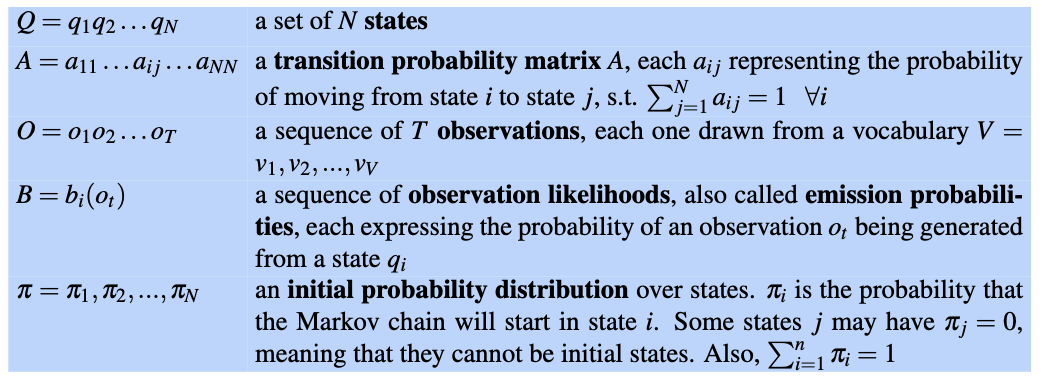
\includegraphics[scale = 0.4]{hmm_notations.png}}
\end{minipage}
\caption{\footnotesize{\textbf{Hidden Markov Model notations}.}}
\label{fig: hmm}
\end{figure}

HMM has two assumptions on the distribution
\begin{itemize}
\item \textbf{Markov assumption}: $P(q_{i}| q_{1},\ldots, q_{i-1}) = P(q_{i}| q_{i-1})$, i.e. given the current state, the future state and the past state are independent. 
\item \textbf{Output Independence}: $P(o_{i}| q_{1},\ldots, q_{i-1}, q_{i}, o_{1}, \ldots, o_{i-1}) = P(o_{i}| q_{i})$, i.e. the current observation is only dependent on the current state.
\end{itemize}

\subsection{HMM for POS tagging}
Part-of-speech tagging can be treated as a decoding problem using HMM, i.e. given HMM $(\mb{A},\mb{B})$ and a sequence of observations (words) $(o_1, \ldots, o_{T})$, find the most probable (maximum a-priori) sequence of states (tags) $(q_{1}, \ldots, q_{T})$ 
\begin{align*}
\hat{q}_{1:T} &= \argmax_{q_{1:T}}P(q_{1:T} | o_{1:T}) \\
&= \argmax_{q_{1:T}}P(o_{1:T} | q_{1:n})P(q_{1:T}) \\
&= \argmax_{q_{1:T}} \prod_{i=1}^{T}P(o_{i}|q_{i})P(q_{i}|q_{i-1})
\end{align*}

\begin{figure}
\begin{minipage}[t]{1\linewidth}
  \centering
  \centerline{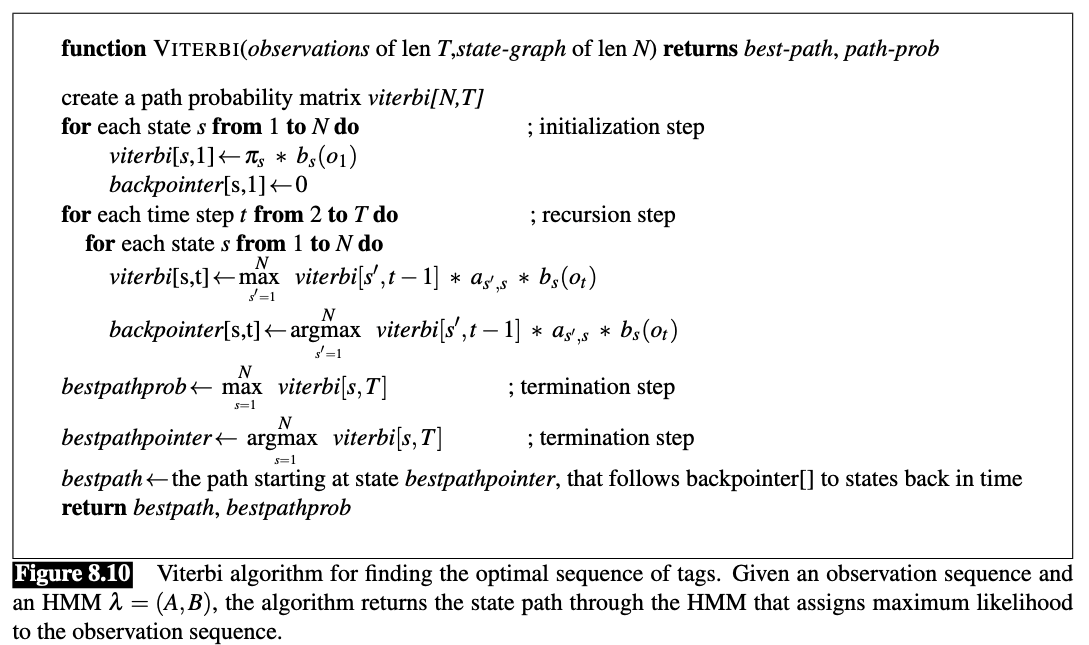
\includegraphics[scale = 0.4]{viterbi_algor.png}}
\end{minipage}
\caption{\footnotesize{\textbf{Viterbi algorithm for decoding HMM}.}}
\label{fig: hmm_decode}
\end{figure}


Solving the optimization problem above can be done via \textbf{Viterbi algorithm}, an instance of \textbf{dynamic programming}. Figure \ref{fig: hmm_decode} describes the Viterbi algorithm. Denote $v_{t}(i)$ being the optimal HMM probability in state $i$ at time $t$ together with stats and observations before $t$, 
\begin{align*}
v_{t}(i) &= \max_{q_{1:t-1}} P(q_{1:t-1}, o_{1:t-1}, q_{t} = i | \lambda)
\end{align*}
The dynamic programming utilize the recursion formula (Bellman equation):
\begin{align}
v_{t}(i) &= \max_{j\in \{1,\ldots,N\}}v_{t-1}(j)\;\; a_{j,i} \;b_{i}(o_{t}) \;\; \label{eqn: bellman_eqn}
\end{align} This choose the most probable \textbf{path probability} based on optimal path from previous stage $t-1$.  

We can compare \eqref{eqn: bellman_eqn} to a linear recursive network. In linear recursive network, the states are updated based on $\mb{v}_{t} = (\mb{A}\mb{v}_{t-1})\odot \mb{B}$. In this equation, we marginalized over all \textbf{path probabilities} (i.e. \textbf{path integral}) to obtain the \emph{marginalized distribution} instead of \emph{posterior} distribution from Viterbi algorithm. In \eqref{eqn: bellman_eqn}, we use max operation $(\max_{j}v_{t-1}(j)a_{j,i})b_{i}$ for each path instead of summation $(\sum_{j}v_{t-1}(j)a_{j,i})b_{i}$ over all paths.


\section{Conditional Random Fields (CRFs)}
HMM is a generative model. It is hard for HMM to add arbitrary features directly into the model. A discriminative model can be better. The \textbf{conditional random field (CRF)} can be used to solve this issue. The most commonly used CRF is linear chain CRF, which is close to HMM. Similar to HMM, CRF optimize the posterior probability
\begin{align*}
\hat{q}_{1:T} &= \argmax_{q_{1:T}} P(q_{1:T} | o_{1:T}).
\end{align*} Unlike HMM, CRF define the conditional probability directly as a \textbf{log-linear} model: 
\begin{align*}
P(q_{1:T} | o_{1:T}) &= \frac{1}{Z(o_{1:T})} \exp\paren{\sum_{k=1}^{K}w_{k}F_{k}(q, o)}\\
&= \frac{1}{Z(o_{1:T})} \exp\paren{\sum_{k=1}^{K}\sum_{t}^{T}w_{k}f_{k}(q_{t}, q_{t-1}, o_{1:T}, t)}\\
\end{align*} Each $f_{k}$ is called a \textbf{local feature}, which is accumulated over time to form a \textbf{global feature} $F_{k}$. Each of local feature is a linear-chain CRF which makes use of the current state/tag $q_{t}$ and previous state/tag $q_{t-1}$ and the entire observations $o_{1:T}$ and the current position $t$. It is linear chain CRG since $f_{k}$ only depends on $q_{t}$ and $q_{t-1}$. An example pos feature $f_{k}:= \ind{o_{t} = \text{"the"}, q_{t} = \text{DET}}$ and 
$f_{s} := \ind{o_{t+1} = \text{"Street"}, q_{t}=\text{PROPN},  q_{t-1}=\text{NUM}}$. For NER feature, could be "identity of $o_{i}$, identity of neighboring words". 

The linear structure of CRF makes it easy to build \textbf{binary feature} and extend to different special cases. These feature can be manually designed or automatically generated via \textbf{feature templates}: $<q_{t}, o_{t}>, <q_{t}, q_{t-1}>, <q_{t}, o_{t-1}, o_{t+1}>$. These features can be generated from training data. For unknown words, we can define the \textbf{word shape} features, which represent the \emph{\textbf{abstract letter pattern}} of the word by mapping lower-case letters to ‘x’, upper-case to ‘X’, numbers to ’d’, and retaining punctuation, e.g. $I.M.F:= X.X.X$. Prefix and suffix features are also useful. For example some feature templates with unknown words such as "$o_i$ contains a particular prefix/suffix" or "$o_{i}$'s word shape" etc.

The \emph{known-word templates} are computed for every word seen in the training set; the \emph{unknown word features} can also be computed for all words in training, or only on training words whose frequency is below some threshold. The result of the known-word templates and word-signature features is \emph{a very large set of features}.

In NER, one feature that is especially useful for \textbf{locations} is a \textbf{gazetteer}, a list of place names, often providing millions of entries for locations with detailed geographical and political information. This can be implemented as a \textbf{binary feature} indicating a phrase appears in the list. Other related resources like name-lists can be used, as can other entity dictionaries like lists of corporations or products, although they may not be as helpful as a gazetteer

\subsection{Inference on CRF}
\begin{align*}
\hat{q}_{1:T} &= \argmax_{q_{1:T}} P(q_{1:T} | o_{1:T})\\
&=  \argmax_{q_{1:T}} \frac{1}{Z(o_{1:T})} \exp\paren{\sum_{k=1}^{K}w_{k}F_{k}(q_{1:T}, o_{1:T})} \\
&=  \argmax_{q_{1:T}}  \exp\paren{\sum_{k=1}^{K}w_{k}F_{k}(q_{1:T}, o_{1:T})} \\
&=  \argmax_{q_{1:T}}  \sum_{k=1}^{K}w_{k}F_{k}(q_{1:T}, o_{1:T}) \\
&=  \argmax_{q_{1:T}}  \sum_{t}^{T}\sum_{k=1}^{K}w_{k}f_{k}(q_{t}, q_{t-1}, o_{1:T}, t) 
\end{align*} Similar to HMM, we can solve the problem using Viterbi algorithm 
\begin{align}
v_{t}(i)&= \max_{j=1,\ldots,N}v_{t-1}(j)\sum_{k=1}^{K}w_{k}f_{k}(q_{t}, q_{t-1}, o_{1:T}, t)    \;\;\label{eqn: CRF_inference}
\end{align} Compared to \eqref{eqn: bellman_eqn}, we can see that the matrix multiplication $\mb{A}\mb{B}$ is replaced by linear combinations of binary features.  

Learning CRF i.e. the weights for global features $\set{w_{k}}$, is a standard supervised learning problem. Given a sequence of observations, feature functions, and corresponding outputs, we use stochastic gradient descent to train the weights to maximize the log-likelihood of the training corpus. 

\section{Recurrent Neural Networks}
We can use simple feed-forward neural network to model the sequence labeling: use a fixed window of size $d$, each time, providing all context words in within the window (centered around a word $w_{i}$) to the feed-forward neural network to predict the label of the word and then slides the window to the right. This method does not handle the sequential nature of the natural languages, thus it fails to capture and exploit the temporal relationships.  

\begin{figure}
\begin{minipage}[t]{1\linewidth}
  \centering
  \centerline{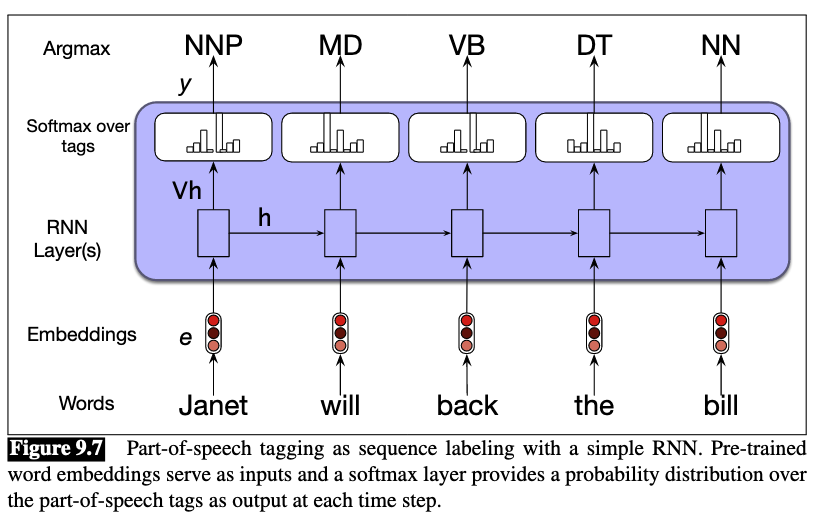
\includegraphics[scale = 0.4]{rnn_inference.png}}
\end{minipage}
\caption{\footnotesize{\textbf{The inference process for RNN on sequence labeling task}.}}
\label{fig: rnn_inference}
\end{figure}

The \textbf{recurrent network (RNN)} offers a new way to represent the prior context, allowing the model’s decision to depend on information from hundreds of words in the past. The transformer offers new mechanisms (self-attention and positional encodings) that help represent time and help focus on how words relate to each other over long distances. 



The inference process of RNN for sequence labeling task is shown below: 
\begin{align*}
\mb{B}_{t} &= \mb{E}\mb{o}_{t} \\
\mb{v}_{t} &= \sigma\paren{\mb{A}\mb{v}_{t-1} + \mb{W}\mb{B}_{t}} \\
\mb{g}_{t} &= \text{softmax}\paren{\mb{U}\mb{v}_{t}}
\end{align*} Here, $\mb{g}_{t}$ is the distribution over tags, and $\mb{o}_{t}$ is a word embedding at position $t$. The state vector $\mb{v}_{t}$. Figure \ref{fig: rnn_inference} illustrate the inference process of RNN on sequence labeling task.


\subsection{LSTM}
In practice, it is quite difficult to train RNNs for tasks that require a network to make use of information distant from the current point of processing. Yet distant information is critical to many language applications.  One reason for the inability of RNNs to carry forward critical information is that the hidden layers, and, by extension, the weights that determine the values in the hidden layer, are being asked to perform two tasks simultaneously: provide information useful for the current decision, and updating and carrying forward information required for future decisions.

The most commonly used extension to RNNs is the \textbf{Long short-term memory (LSTM)} network. LSTMs divide the context management problem into two sub-problems: \emph{removing information no longer needed from the context}, and \emph{adding information likely to be needed for later decision making}. The key to solving both problems is to learn how to manage this context rather than hard-coding a strategy into the architecture. 

LSTMs accomplish this by first adding an explicit \emph{context layer} to the architecture (in addition to the usual \emph{recurrent hidden layer}), and through the use of specialized neural units that make use of \textbf{gates} to control the flow of information into and out of the units that comprise the network layers. These gates are implemented through the use of additional weights that operate sequentially on the input, and \emph{previous hidden layer}, and \emph{previous context layers}.

\begin{figure}
\begin{minipage}[t]{1\linewidth}
  \centering
  \centerline{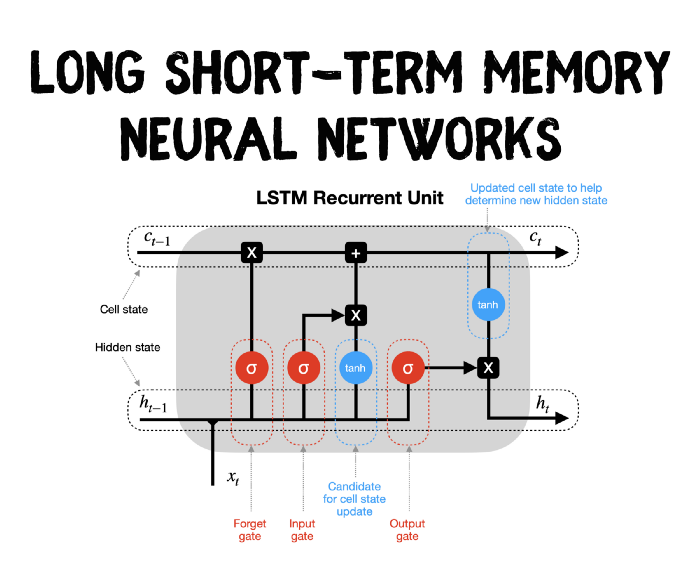
\includegraphics[scale = 0.5]{LSTM.png}}
\end{minipage}
\caption{\footnotesize{\textbf{The Long Short Term Memory}.}}
\label{fig: lstm}
\end{figure}

LSTM structure can be divided into several parts (see Figure \ref{fig: lstm}):
\begin{itemize}
\item \textbf{forget gate}: The purpose of this gate to \textbf{delete information from the context} that is no longer needed.
\begin{align*}
\mb{f}_{t} &= \sigma\paren{\mb{U}_{f}\mb{h}_{t-1} + \mb{W}_{f}\mb{x}_{t}} 
\end{align*} where $\mb{x}_{t}$ is the input observation, $\mb{h}_{t-1}$ is the recurrent hidden layer (short memory) at $t-1$, and $\mb{c}_{t}$ is the context layer (long memory). $\sigma(\cdot)$ is the sigmoid function output $[0,1]$.

\item \textbf{input gate}: The purpose of this gate is to select the information to \textbf{add to the current context}.
\begin{align*}
\mb{i}_{t} &= \sigma\paren{\mb{U}_{i}\mb{h}_{t-1} +  \mb{W}_{h}\mb{x}_{t}}
\end{align*}

\item \textbf{candidate for context update}: 
\begin{align*}
\mb{g}_{t} &= \text{tanh}\paren{\mb{U}_{g}\mb{h}_{t-1} + \mb{W}_{g}\mb{x}_{t}}
\end{align*}


\item \textbf{context update}: The context (long-term memory) is determined by combination of its previous context masked by forget gate and the current hidden state candidate masked by input gate
\begin{align*}
\mb{c}_{t} &= \mb{f}_{t}\odot \mb{c}_{t-1} + \mb{i}_{t}\odot \mb{g}_{t}
\end{align*}


\item \textbf{output gate}: This gate is used to decide what information is required for the \textbf{current hidden state} (as opposed to what information needs
to be \emph{preserved for future decisions}).
\begin{align*}
\mb{o}_{t} &= \sigma\paren{\mb{U}_{o}\mb{h}_{t-1} +  \mb{W}_{o}\mb{x}_{t}}
\end{align*}

\item \textbf{hidden (recurrent) state update}: the updated hidden (recurrent) state is determined by output gate and context vector (long-term memory)
\begin{align*}
\mb{h}_{t} &= \mb{o}_{t}\odot \text{tanh}\paren{\mb{c}_{t}}
\end{align*}
\end{itemize}

As seen in Figure \ref{fig: lstm}, the hidden recurrent state (short-term memory) at previous stage $\mb{h}_{t-1}$ and input $\mb{x}_{t}$ at current stage jointly determined the \emph{forget gate}, the \emph{input gate}, the \emph{output gate} and the \emph{candidate context}. Thus $\mb{h}_{t-1}$,  $\mb{x}_{t}$ and the previous stage $\mb{c}_{t-1}$ jointly determine the long-term memory $\mb{c}_{t}$ at current stage. The long-term memory $\mb{c}_{t}$ and the output gate (thus $\mb{h}_{t-1}$ and  $\mb{x}_{t}$) determine the short-term memory  $\mb{h}_{t}$ at current stage. 


\section{Transformer}
LSTM still not fully resolve the challenges of long dependencies and vanishing gradient problem. Passing information through an extended series of recurrent connections leads to information loss and difficulties in training. Moreover, the inherently sequential nature of recurrent networks makes it hard to do computation in \emph{parallel}. In \citep{vaswani2017attention},  it introduces an encoder-decoder architecture based on \emph{attention layers}, termed as the \textbf{transformer}. One main difference is that the input sequence can be passed parallelly so that GPU can be utilized effectively, and the speed of training can also be increased. And it is based on the multi-headed attention layer, vanishing gradient issue is also overcome by a large margin. 

Transformers map sequences of input vectors $(\mb{x}_1, \ldots, \mb{x}_n)$ to sequences of output vectors $(y_1, \ldots y_n)$ of the same length.  Transformers are made up of stacks of transformer blocks, which are multilayer networks made by combining simple linear layers, feedforward networks, and \textbf{self-attention layers}, the key innovation of transformers. Self-attention allows a network to directly extract and use information from arbitrarily large contexts without the need to pass it through intermediate recurrent connections as in RNNs. 

\begin{figure}
\begin{minipage}[t]{1\linewidth}
  \centering
  \centerline{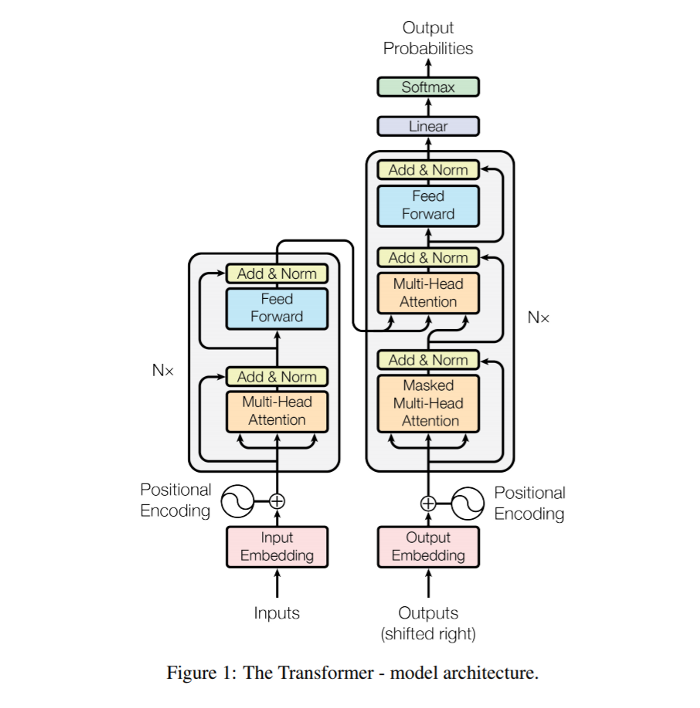
\includegraphics[scale = 0.4]{transformer.png}}
\end{minipage}
\caption{\footnotesize{\textbf{The encoder-decoder structure of transformer}.}}
\label{fig: transformer_block}
\end{figure}



At the core of an attention-based approach is the ability to \textbf{\emph{compare}} an item of interest to a collection of other items in a way that reveals their relevance in the current context. In the case of self-attention, the set of comparisons are to other elements within a given sequence. The result of these comparisons is then used to
compute an output for the current input. The attention score is computed using softmax of inner product between two inputs:
\begin{align*}
\alpha_{i,j}&= \text{softmax}(\mb{x}_{i}^{T}\mb{x}_{j})\nonumber\\
&= \frac{\exp(\mb{x}_{i}^{T}\mb{x}_{j})}{\sum_{k}\exp(\mb{x}_{i}^{T}\mb{x}_{k})}
\end{align*} $\alpha_{i, j}$ indicates the proportional relevance of each input to the input element $i$ that is the current focus of attention. And the output can be seen as linear combination of inputs weighted by attention score 
\begin{align*}
\mb{y}_{i} &= \sum_{j}\alpha_{i,j}\mb{x}_{j}.
\end{align*} The result of a dot product can be an arbitrarily large (positive or negative) value. Exponentiating such large values can lead to numerical issues and to an effective loss of gradients during training. To avoid this, the dot product needs to be \emph{scaled} in a suitable fashion. A scaled dot-product approach divides the result of the dot product by a factor related to the size of the embeddings before passing them through the softmax. A typical approach is to divide the dot product by the square root of the
dimensionality of the query and key vectors $d_{k}$. 
\begin{align*}
\alpha_{i,j}&= \text{softmax}\paren{\frac{\mb{x}_{i}^{T}\mb{x}_{j}}{\sqrt{d_{k}}}}
\end{align*}



The core of an attention-based approach includes:
\begin{itemize}
\item a set of comparisons to relevant items in some context, 
\item a normalization of those scores to provide a probability distribution
\item a weighted sum using this distribution. The output $\mb{y}$ is the result of this straightforward computation over the inputs.
\end{itemize} 

Transformers allow us to create a more sophisticated way of representing how words can contribute to the representation of longer inputs. Consider the three
different \emph{\textbf{roles}} that each input embedding plays during the course of the attention process.
\begin{itemize}
\item As the \emph{current} \emph{focus} of attention when being compared to all of the other preceding inputs. This role is refer to as a \textbf{query}.
\item In its role as a preceding input \emph{being compared to} the current focus of attention. This role is refer to as a \textbf{key}.
\item And finally, as a \textbf{value} used to compute the output for the current focus of attention.
\end{itemize} To capture these three different roles, transformers introduce weight matrices $\mb{W}_Q \in \bR^{d_{k}\times d}$, $\mb{W}_K \in \bR^{d_{k}\times d}$, and $\mb{W}_V \in \bR^{d_{v}\times d}$. These weights will be used to project each input vector $\mb{x}_i \in \bR^{d}$ into a representation of its role as a key, query, or value.
\begin{align*}
\mb{q}_{i} = \mb{W}_{Q}\mb{x}_{i},\;\;\mb{k}_{i} = \mb{W}_{K}\mb{x}_{i},\;\;\mb{v}_{i} = \mb{W}_{V}\mb{x}_{i}
\end{align*} The attention score is computed between key and query 
\begin{align}
\alpha_{i,j}&= \text{softmax}\paren{\frac{\mb{q}_{i}^{T}\mb{k}_{j}}{\sqrt{d_{k}}}}  \label{eqn: attention_comp}
\end{align} Each output $\mb{y}_{i}$ can be computed in parallel by taking advantage of efficient matrix multiplication routines. Let $\mb{X} \in \bR^{N \times d}$ be the input matrix with each row being the embedding of word $i$. Then we can compute the query $\mb{Q} \in \bR^{N \times d_{k}}$, key $\mb{K} \in \bR^{N \times d_{k}}$ and value matrix  $\mb{V} \in \bR^{N \times d_{v}}$ via 
\begin{align*}
\mb{Q} = \mb{X}\mb{W}^{T}_{Q},\;\;\mb{K} = \mb{X}\mb{W}^{T}_{K},\;\;\mb{V} = \mb{X}\mb{W}^{T}_{V}
\end{align*} Given these matrices we can compute all the requisite query-key comparisons \textbf{simultaneously} by multiplying $\mb{Q}$ and $\mb{K}^{T}$ in a single matrix multiplication.  Taking this one step further, we can scale these scores, take the softmax, and then multiply the result by $\mb{V}$ resulting
in a matrix of shape $N \times d_{v}$: a \emph{vector embedding representation} for each token in the
input. 
\begin{align}
\text{self-attention}(\mb{Q}, \mb{K},  \mb{V}) &= \text{softmax}\paren{\frac{\mb{Q}\mb{K}^{T}}{\sqrt{d_{k}}}}\mb{V}\;\;\;\;\; \in \bR^{N\times d_{v}} \label{eqn: self_attention_mat}
\end{align} The $N\times N$ self-attention comparison matrix can be \textbf{masked}, e.g. to cover all entries in upper triangle with $-\infty$ to avoid knowing words ahead of current word. Computation of this $N\times N$ takes quardratic time which is very expensive for long input sentences. 


\subsection{Transformer blocks}
The self-attention calculation lies at the core of what’s called a \emph{transformer block}, which, in addition to the self-attention layer, includes additional feedforward layers,
residual connections, and normalizing layers. The input and output dimensions of these blocks are matched so they can be stacked just as was the case for stacked
RNNs. 

A transformer block consists of following components:
\begin{itemize}
\item a self-attention layer with residual connections followed by layer normalization:
\begin{align*}
\mb{z} &= \text{LayerNorm}\paren{\mb{x} + \text{SelfAttn}(\mb{x})}
\end{align*}

\item a feed-forward layer with residual connections followed by layer normalization:
\begin{align*}
\mb{y} &= \text{LayerNorm}\paren{\mb{z} + \text{FFNN}(\mb{z})}
\end{align*}
\end{itemize}

In deep networks, \textbf{residual connections} \citep{he2016deep} are connections that pass information from a lower layer to a higher layer without going through the intermediate layer. Allowing information from the activation going forward and the gradient going backwards to skip a layer improves learning and gives higher level layers direct access to information from lower layers.


\textbf{Layer normalization} (or \textbf{layer norm}) is one of many forms of normalization that can be used to improve training performance in deep neural networks by keeping the values of a hidden layer in a range that facilitates gradient-based training. Layer norm is a variation of the standard score, or \textbf{z-score}, from statistics applied to a single hidden layer. 
\begin{align*}
\hat{x}_{i} &= \frac{(x_{i} - \mu)}{\sigma} \\
\text{where } \mu &= \frac{1}{d_{h}}\sum_{i}x_{i} \\
 \sigma &= \sqrt{\frac{1}{d_{h}}\sum_{i}(x_{i} - \mu)^{2}}. \\
  \text{LayerNorm}(\mb{x}) &= \gamma \hat{\mb{x}} + \beta,
\end{align*} where $\gamma$ and $\beta$ are two learnable parameters.

\begin{figure}
\begin{minipage}[t]{1\linewidth}
  \centering
  \centerline{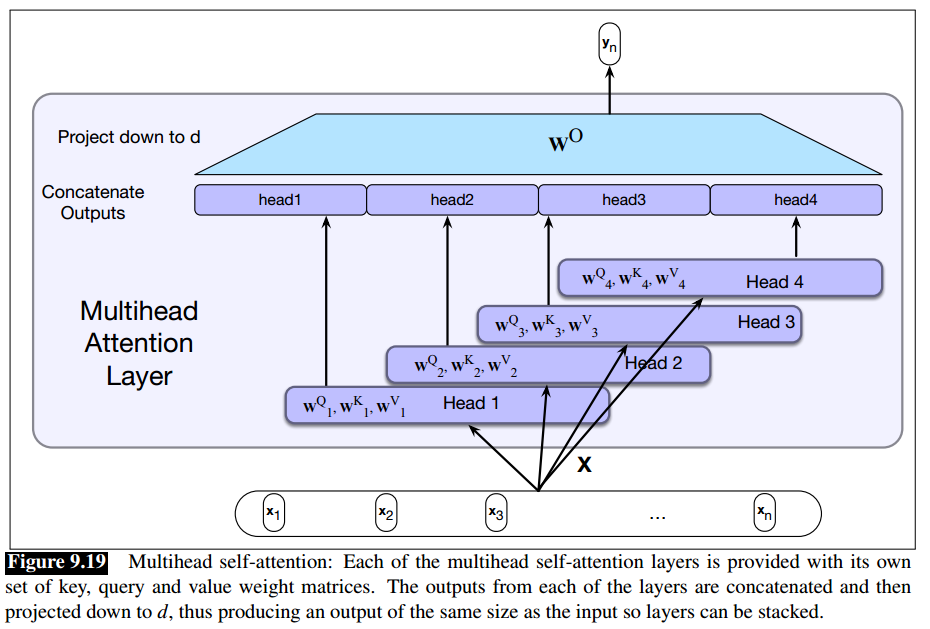
\includegraphics[scale = 0.4]{multi-head-attn.png}}
\end{minipage}
\caption{\footnotesize{\textbf{The multi-head attention}.}}
\label{fig: multi-head-attn}
\end{figure}

\subsection{Multi-head attention}
The different words in a sentence can relate to each other in many different ways \emph{simultaneously}. For example, distinct syntactic, semantic, and discourse relationships
can hold between verbs and their arguments in a sentence. It would be difficult for a single transformer block to learn to capture all of the different kinds of parallel
relations among its inputs. Transformers address this issue with \textbf{multihead self-attention layers}. These are sets of self-attention layers, called \textbf{heads}, that reside in parallel layers at the same depth in a model, each with its own set of parameters. Given these distinct sets of parameters, each head can learn \emph{different aspects of the relationships} that exist among inputs at the same level of abstraction.  Figure \ref{fig: multi-head-attn} illustrate the approach. 

To implement this notion, each head, $i$, in a self-attention layer is provided with its own set of key, query and value matrices $\mb{W}^{i}_Q \in \bR^{d_{k}\times d}$, $\mb{W}^{i}_K \in \bR^{d_{k}\times d}$, and $\mb{W}^{i}_V \in \bR^{d_{v}\times d}$. These are used to project the inputs into separate key, value, and query embeddings separately for each head, with the rest of the self-attention computation remaining unchanged.  The output of each of the $h$ heads is of shape $N \times d_v$, and so the output of the multi-head layer with $h$ heads consists of $h$ vectors of shape $N \times d_v$. To make use of these vectors in further processing, they are combined and then reduced down to the original input dimension $d$. This is accomplished by \textbf{concatenating} the outputs from each \emph{head} and then using yet another linear projection, $\mb{W}_O \in \bR^{h\,dv\times d},$ to reduce it to the original output dimension for each token, or a total $N \times d$ output
\begin{align*}
\text{MultiHeadAttn}(\mb{X}) &= \paren{\mb{head}_1 \oplus \ldots \oplus \mb{head}_h }\mb{W}_{O} \quad \in \bR^{N \times d} \\
\mb{head}_i(\mb{Q}_{i}, \mb{K}_{i},  \mb{V}_{i}) &=  \text{softmax}\paren{\frac{\mb{Q}_{i}\mb{K}_{i}^{T}}{\sqrt{d_{k}}}}\mb{V}_{i} \quad \in \bR^{N \times d_{v}} \\
\text{where }&\mb{Q}_{i} = \mb{X}(\mb{W}^{i}_{Q})^{T},\;\;\mb{K}_{i} = \mb{X}(\mb{W}^{i}_{K})^{T},\;\;\mb{V}_{i} = \mb{X}(\mb{W}^{i}_{V})^{T}
\end{align*}




\subsection{Modeling word order: positional embeddings}
The attention mechanism itself does not contain information on the relative, or absolute positions of the tokens in the input.  One simple solution is to modify the input embeddings by combining them with \textbf{positional embeddings} specific to each position in an input sequence.

\begin{figure}
\begin{minipage}[t]{1\linewidth}
  \centering
  \centerline{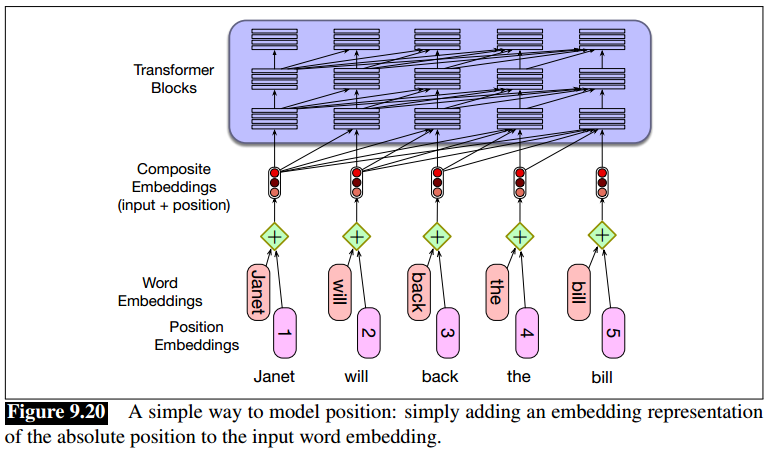
\includegraphics[scale = 0.4]{pos_embedding.png}}
\end{minipage}
\caption{\footnotesize{\textbf{The simple way to implement positional embedding}.}}
\label{fig: pos_embedding}
\end{figure}

A simple implementation of postitional embedding is to add word embedding with the embedding of the position index, as shown in Figure \ref{fig: pos_embedding}. A potential problem with the simple \emph{\textbf{absolute position} embedding approach} is that there will be plenty of training examples for the initial positions in our inputs and
correspondingly \textbf{fewer at the outer length limits}. An alternative approach to positional embeddings is to choose a \emph{static function} that maps integer inputs to real-valued vectors in a way that \textbf{captures the inherent relationships among the positions}. That is, it captures the fact that position $4$ in an input is more closely related to position $5$ than it is to position $17$. A combination of \emph{sine} and \emph{cosine functions} with differing frequencies (\textbf{Fourier transform}) was used in the original transformer work. Developing better position representations is an ongoing research topic.


\subsection{Encoder-Decoder structure}

Figure \ref{fig: transformer_block} shows the architecture of transformer used for sequence-to-sequence task such as machine translation, text summarization, question answering. 



\begin{figure}
\begin{minipage}[t]{1\linewidth}
  \centering
  \centerline{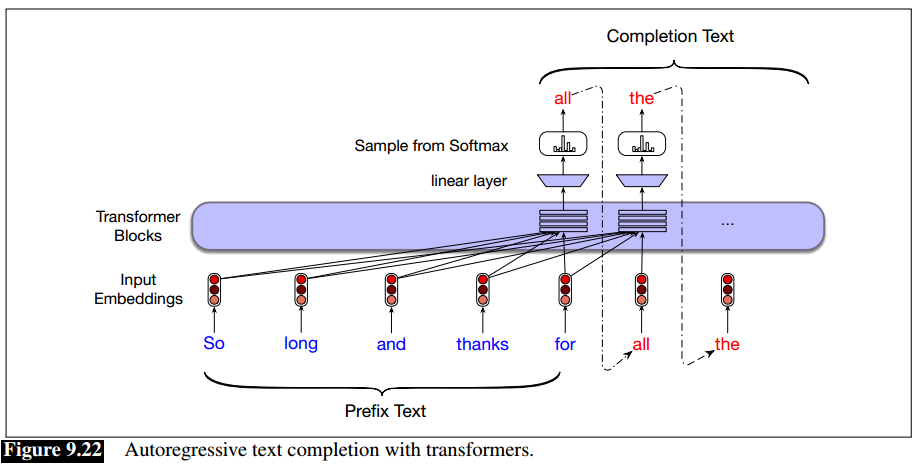
\includegraphics[scale = 0.4]{autoregressive_text.png}}
\end{minipage}\\
\begin{minipage}[t]{1\linewidth}
  \centering
  \centerline{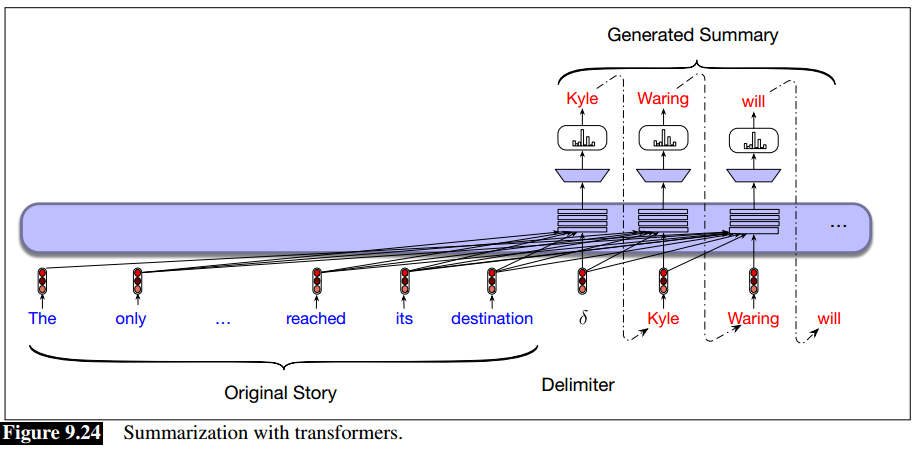
\includegraphics[scale = 0.4]{text_summarization.png}}
\end{minipage}
\caption{\footnotesize{\textbf{The autoregressive text generation using transformer}.}}
\label{fig: auto_text}
\end{figure}

\subsection{Transformer for Contextual Generation and Summarization}
A simple variation on autoregressive generation that underlies a number of practical applications uses a prior context to prime the autoregressive generation process. Figure \ref{fig: auto_text} describes an auto-regressive process to generate text based on context. Here a standard language
model is given the \textbf{prefix} to some text and is asked to generate a possible completion to it. Note that as the generation process proceeds, the model has direct access to the \emph{priming context} as well as to all of \emph{its own subsequently generated outputs}. This ability to incorporate the entirety of the \emph{earlier context and generated outputs} at each time step is the \textbf{key} to the power of these models.

\textbf{Text summarization} is a practical application of context-based autoregressive generation. The task is to take a full-length article and produce an effective summary
of it. A simple but surprisingly effective approach to applying transformers to summarization is to \textbf{append} a \emph{summary} to each full-length article in a \emph{corpus}, with a unique \emph{\textbf{marker}} separating the two. More formally, each article-summary pair $(\mb{x}_1, \ldots, \mb{x}_n)$ , $(y_1, \ldots y_n)$ in a training corpus is converted into a single training instance $(\mb{x}_1, \ldots, \mb{x}_n, \delta, y_1, \ldots y_n)$ with an overall length of $n+ m+ 1$. These training instances
are treated as long sentences and then used to train an autoregressive language model using \textbf{teacher forcing}, exactly as we did earlier.

Once trained, full articles ending with the special marker are used as the context to prime the generation process to produce a summary as illustrated in Figure \ref{fig: auto_text}.




\newpage
\bibliographystyle{plainnat}
\bibliography{book_reference.bib}
\end{document}